\section{Theoretical Guarantees of EMA}

In this section, we show that EMA preserves the asymptotic complexity of the base index in terms of both construction time and index size.
We also derive the local deletion-work bound stated in Section~4.1 of the main paper.
We further analyze the source of false positives introduced by Markers and provide theoretical bounds on the false positive rate.



\subsection{Complexity}

% Although Marker propagation modifies the index construction procedure and increases the memory footprint, we prove that the asymptotic time complexity of index construction remains unchanged.


\begin{lemma}[Cost of MEncode and edge existance]
In Algorithm~3, \texttt{MEncode} takes
$O(m)$ time. Testing whether $e_{(n,v)}$ previously exists takes $O(M)$ time,
since it scans at most $M$ previously stored neighbors.
\label{le:mencode}
\end{lemma}

\begin{theorem}
The time complexity of Algorithm~3 is
\[
O\!\left(efc \cdot M \cdot (M+m)\right).
\]
\end{theorem}

\begin{proof}
The outer loop iterates over candidates $v\in Cand$, so it executes at most
$|Cand|\le efc$ times.

For a fixed candidate $v$, the inner loop scans $u\in Nbrs$. The neighbor list is
bounded by the maximal size $M$, hence $|Nbrs|\le M$ and the inner loop runs at most
$M$ times.

Consider one inner-loop iteration for a pair $(u,v)$. Besides a constant-time distance
comparison, when $u$ dominates $v$ the algorithm (i) tests whether $e_{(n,v)}$ previously exists,
which costs $O(M)$, and then (ii) calls either Marker merge or \texttt{MEncode},
which costs $O(m)$ by Lemma~\ref{le:mencode}. Therefore, each inner-loop iteration costs $O(M+m)$ in the worst case.

Thus, for each candidate $v$, the inner loop costs
\[
O\!\left(M\cdot(M+m)\right).
\]
The remaining work per candidate (insertion into $Nbrs$ and one additional
\texttt{MEncode}) is at most $O(M+m)$ and is dominated by the inner-loop bound.
Summing over all $|Cand|\le efc$ candidates gives
\[
O\!\left(efc \cdot M \cdot (M+m)\right).
\]
\end{proof}



The time complexity of HNSW index construction is empirically close to $O(n \log n)$ and is highly correlated with the parameters $M$ and $efc$, which can be expressed as $O(M \cdot efc \cdot n \log n)$.
In our method, Marker propagation introduces additional operations, resulting in a complexity of $O(M \cdot (M + m) \cdot efc \cdot n \log n)$.
However, since both $M$ and $m$ are constants that are significantly smaller than $n$, the asymptotic time complexity remains unchanged.


\begin{theorem}
The space complexity of EMA is
\[
O(nM\cdot sm),
\]
\end{theorem}

\begin{proof}
The additional storage introduced by EMA consists of the Marker stored per neighbor (edge), which is only used in the bottom layer.

In the bottom layer, each of the $n$ nodes stores at most $M$ neighbors, resulting in at most $nM$ edges.
Each edge stores a Marker of size $sm$ bits, so the total Marker storage is
\[
(nM)\cdot sm\ \text{bits}.
\]

The top layer contains at most $n$ nodes, each with at most $M$ outgoing edges.
It stores no Markers and contributes $O(nM)$ space.

Combining both parts yields a total space complexity of
\[
O\!\left(nM\cdot sm + nM\right),
\]
which simplifies to $O(Mn\cdot sm)$.
\end{proof}

\paragraph{Deletion complexity.}
We analyze the local graph and Marker maintenance procedure for deleting one point $a$ in the main paper's Marker-aware Deletion algorithm.
Let $n$ denote the number of stored points, including retained deleted records.
We retain the degree parameter $M$, search width $efc$, and attribute count $m$.
Vector dimension, per-attribute encoding capacities, and the reconnection budgets $k_r=50$, $c=3$ are fixed.
Thus a distance evaluation costs $O(1)$, while a full Marker operation or \texttt{MEncode} costs $O(m)$.
We use the parameterized search model of the construction analysis: navigation and each layer search examine $O(efc\log n)$ rows of degree $O(M)$, at cost $O(M\cdot efc\log n)$ including bounded-queue bookkeeping.
Identifier-keyed work lists use the standard expected amortized $O(1)$ model for dictionary lookup and insertion.
We count the logical graph and Marker procedure; request compatibility can be evaluated directly over its bounded witness context, without requiring memoization.

\begin{lemma}[Deletion complexity]
\label{le:deletion-cost}
Under the stated search and dictionary models, the expected work of one local deletion is
\begin{equation}
O\!\left(M \cdot efc \cdot (M+efc\cdot m)\log n\right).
\label{eq:app-deletion-local}
\end{equation}
\end{lemma}

\begin{proof}
\emph{Search and discovery.}
IP-DiskANN's Algorithm~5 searches with the old vector and checks examined adjacency lists for incoming edges~\cite{xu2025ipdiskann}.
By the adopted model, the constant number of layer searches and incoming-edge scans costs $O(M\cdot efc\log n)$.
At most $O(efc\log n)$ incoming sources are discovered.
The outgoing pass issues $O(cM)$ proposals, but their source IDs all come from the same first $k_r$ retained candidates, so it adds only $O(1)$ distinct source rows.
Proposals are merged by source and layer, and each repair plan executes once.
Thus the number $r_a$ of reconstructed adjacency rows across both layers is $O(efc\log n)$.
This bounds discovered repair rows, not the deleted point's full in-degree.

\emph{Work per repaired row.}
Each source receives $O(M)$ old targets, at most $c$ incoming-side replacements, and $O(M)$ outgoing-side targets, giving an $O(M)$ target pool.
Selecting replacements scores at most the first $k_r$ retained candidates, rather than launching a fresh graph search for each source.
Pool formation, duplicate checks, ranking, and RNG comparisons cost $O(M^2)$ per row.
Here pruning records direct witness IDs rather than propagating historical Markers; each pruned candidate is assigned to at most one owner.
Coverage admission, old-Marker preservation, and direct-witness encoding therefore add $O(Mm)$.
All base-layer repairs share the deletion's witness context, which contains at most $efc$ candidates.
For $O(M)$ owners, testing request compatibility and coverage against those witnesses costs $O(M\cdot efc\cdot m)$.
The total per repaired row is consequently $O(M^2+M\cdot efc\cdot m)$.

\emph{Context and nonincident Marker cleanup.}
Encoding the retained candidates and building their support lists costs $O(efc\cdot m)$.
Cleanup applies to at most $efc$ retained source rows.
Each such source inspects $O(M)$ neighbors to select one dominator, then checks that owner's removable bits against at most $efc$ witnesses.
This costs $O((M+efc)m)$ per source and $O(efc(M+efc)m)$ in total.

\emph{Aggregation.}
Identifier lookup and work-list management use the stated expected constant-time dictionary model; target-pool edits have already been charged above.
Publishing each row and its Markers costs $O(Mm)$, also covered by the per-row bound.
There are no concurrent point workers or deferred inter-point repair searches for this single-point procedure.
Writing $T_a$ for the expected local work and substituting $r_a=O(efc\log n)$ gives
\[
\begin{aligned}
T_a = O\!\Bigl(&M\cdot efc\log n + efc(M+efc)m\\
              &+(1+r_a)(M^2+M\cdot efc\cdot m)\Bigr)\\
    = O\!\Bigl(&M\cdot efc\cdot(M+efc\cdot m)\log n\Bigr),
\end{aligned}
\]
which proves Equation~\eqref{eq:app-deletion-local}.
\end{proof}

For fixed $M$, $efc$, and $m$, this is $O(\log n)$.
As in the construction analysis, this is a local-algorithm bound under the stated models, not an unconditional worst-case traversal or implementation-level guarantee.

\paragraph{Reconnection details.}
Each incoming- or outgoing-side proposal ranks the original first $k_r=50$
retained candidate positions and admits at most $c=3$ eligible endpoints.
Invalid or retired endpoints, the deleted point, and the affected endpoint are
excluded without widening that prefix.
The deleted point's native placeholder still consumes its original rank.

\paragraph{RNG dominance and Marker cleanup.}
On a Marker-bearing layer, let $F(x)={\tt MEncode}(x.A,\mathcal C)$
under the fixed Codebook $\mathcal C$, and let $Cand$ denote the
retained layer-search candidates.
For source $u$, neighbor $v$, and candidate $w$, define
\[
  D(u,v,w)\equiv
  dis(u,v)\le dis(u,w)\land dis(v,w)<dis(u,w).
\]
The first comparison captures the distance ordering in RNG pruning;
the second is its domination test.
Nonincident Marker cleanup applies only to retained live candidate sources;
examined-only rows may receive graph repair without this cleanup.
For a deleted point $a$ and each such source $u$, select the live neighbor
$v$ closest to $u$ among those satisfying $D(u,v,a)$.
If no such neighbor exists, no nonincident Marker is cleaned for that source.
Equal-distance ties between valid cleanup owners follow adjacency-row order.
The candidate bits for clearing are
\[
  e_{(u,v)}.\mathrm{Marker}\land F(a)\land\neg F(v).
\]
Clear a set bit $b$ of this mask only when no live
$w\in Cand\setminus\{a,u,v\}$ has both $F(w)[b]=1$ and $D(u,v,w)$.
Thus the target's own encoding and bits supported by retained live witnesses
are protected.
Reconstruction uses the same $D(u,v,w)$ when testing whether a selected owner
already covers $F(w)$ and when choosing a compatible requesting owner for $w$.
This is a current geometric compatibility test, not a recovery of exact
historical pruning assignments.

\paragraph{Batched deletion and cross-point repair.}
The main paper's Marker-aware Deletion algorithm describes one logical point
deletion. The batched implementation may execute several such point tasks in
parallel.
A repair can encounter another target that is being retired by a different
task. It hands the source ID, layer, and optional Marker-recovery request to the
active deletion task for that target.
The recipient applies incoming repair deltas using its retained layer
candidates. Closing a task is synchronized with outstanding producers so that
reserved requests are not lost.
Valid requests that arrive after the recipient has closed enter a batch-local
deferred queue; completion epochs distinguish overlapping work from
already-completed stale edges.

Deferred repairs may search again at width $efc$ to construct a fresh bounded
witness context and can generate further repair handoffs.
Each producing worker services deferred work before returning, and the batch
waits for its workers and their claimed repairs to finish.
These repairs complete within the deletion call rather than waiting for a
subsequent query.
Liveness is rechecked when using witnesses and publishing edges.
Callers must prevent external queries and mutations from overlapping this
stop-the-world operation; parallelism is internal to the deletion batch.
The single-point complexity bound above does not include this cross-point
coordination or its additional repair searches.

\subsection{Theoretical Analysis of Marker False Positives}

% A key challenge in early filtering using Marker is the presence of Marker-matched nodes that do not satisfy the predicate, causing \emph{false positives}.
% Marker false positives arise in two cases:
% (1) attribute information merged from dominated nodes differs from that of the dominating node; and
% (2) the query predicate does not fully align with the granularity of the Codebook.
% For example, if a codebook entry $\mathcal{C}_1[1]$ corresponds to the range $[0,10)$, then a query predicate $[5,6]$ will match the corresponding Marker, even though the Marker is activated by an attribute value of $4$.

% Case (1) is empirically beneficial, as it enables navigation toward nearby predicate-matched nodes.
% Although the size of the dominated region is not theoretically bounded, such false positives typically guide the search in a correct direction.
% In contrast, Case (2) is more problematic, as it may direct the search toward regions that contain no nodes satisfying the predicate, purely due to the mismatch between predicate granularity and the Marker Codebook.

% Yang et al.~\cite{yang2025esg} show that when predicate selectivity is no less than 50\%, the performance of post-filtering does not degrade significantly.
% While post-filtering and joint filtering differ in their execution models, this observation provides a useful reference point for assessing the impact of false positives in joint filtering. 

% We study the two sources of Marker false positives separately: for Case (1), we derive an average-case characterization based on the
% expected dominate size; for Case (2), we establish a sufficient bound to control Codebook-induced false positives.

\begin{definition}[Expected Case-(1) False Positive Rate]
\label{def:case1-fpr}
Consider a directed edge $e_{(u,v)}$ whose Marker is constructed by aggregating the attribute bitmaps of the dominating node $v$ and the set of nodes dominated by $v$ with respect to $u$, denoted by $D(e)$; hence $v \notin D(e)$.

Let $R$ be a query predicate with selectivity $\mathrm{sel}$, i.e., for a randomly drawn node $p$,
\[
\Pr[p \models R] = \mathrm{sel},
\]
and assume that, conditional on the graph, predicate satisfaction events are
independent and identically distributed across nodes.

A \emph{Case-(1) false positive} occurs on edge $e$ if the Marker is activated due to at least one dominated node satisfying the predicate, while the target node itself does not satisfy the predicate. Formally,
\[
\mathrm{FP}_{\mathrm{case1}}(e)
\iff
\big(v.A \not\models R\big)
\;\wedge\;
\Big(\exists p \in D(e): p \models R\Big).
\]
This event requires a predicate-matching dominated node; it does not count
aggregate matches assembled from different nodes across predicate components.
\end{definition}

\begin{theorem}[Expected Case-(1) False Positive Rate]
\label{thm:case1}
Let $|D(e)|$ denote the dominate size of edge $e$, and let
\[
\mu = \mathbb{E}[\,|D(e)|\,]
\]
be the average dominate size over all edges.

Under the assumptions of Definition~\ref{def:case1-fpr}, the expected false positive rate induced by Case~(1) is given by
\[
\mathrm{FPR}_{\mathrm{case1}}
=
(1-\mathrm{sel}) \cdot
\Big(1 - \mathbb{E}\big[(1-\mathrm{sel})^{|D(e)|}\big]\Big).
\]

Moreover, the false positive rate admits the following upper bound that depends only on the average dominate size $\mu$:
\[
0
\;\le\;
\mathrm{FPR}_{\mathrm{case1}}
\;\le\;
(1-\mathrm{sel}) \cdot \big(1-(1-\mathrm{sel})^{\mu}\big).
\]

In particular, under the common average-size approximation $|D(e)| \approx \mu$, we obtain
\[
\mathrm{FPR}_{\mathrm{case1}}
\;\approx\;
(1-\mathrm{sel}) \cdot \big(1-(1-\mathrm{sel})^{\mu}\big).
\]
\end{theorem}


\begin{proof}
By definition, a Case-(1) false positive occurs when the Marker of an edge $e=(u\!\to\!v)$ is activated due to at least one dominated node satisfying the query predicate, while the target node $v$ itself does not satisfy the predicate. Formally, the event is
\[
\mathrm{FP}_{\mathrm{case1}}(e)
\iff
\big(v.A \not\models R\big)
\;\wedge\;
\Big(\exists p \in D(e): p \models R\Big).
\]

Conditioned on a fixed dominate size $|D(e)| = k$, independence implies
\[
\Pr[v.A \not\models R] = 1-\mathrm{sel},
\]
and
\[
\Pr\big(\exists p \in D(e): p \models R\big)
= 1 - \Pr\big(\forall p \in D(e): p \not\models R\big)
= 1 - (1-\mathrm{sel})^{k}.
\]
Since the two events are independent, we obtain
\[
\Pr(\mathrm{FP}_{\mathrm{case1}} \mid |D(e)|=k)
= (1-\mathrm{sel}) \cdot \big(1-(1-\mathrm{sel})^{k}\big).
\]

Taking expectation over the random variable $|D(e)|$ yields
\[
\Pr(\mathrm{FP}_{\mathrm{case1}})
= (1-\mathrm{sel}) \cdot
\Big(1 - \mathbb{E}\big[(1-\mathrm{sel})^{|D(e)|}\big]\Big).
\]

To derive a bound that depends only on the average dominate size
$\mu = \mathbb{E}[|D(e)|]$, observe that the function
$f(k) = (1-\mathrm{sel})^{k}$ is convex for $k \ge 0$.
By Jensen's inequality,
\[
\mathbb{E}\big[(1-\mathrm{sel})^{|D(e)|}\big]
\;\ge\;
(1-\mathrm{sel})^{\mathbb{E}[|D(e)|]}
=
(1-\mathrm{sel})^{\mu}.
\]
Substituting this inequality gives
\[
\mathrm{FPR}_{\mathrm{case1}}
\le
(1-\mathrm{sel}) \cdot \big(1-(1-\mathrm{sel})^{\mu}\big).
\]
Non-negativity of probabilities establishes the lower bound.
\end{proof}


\paragraph{Example.}
At $\mathrm{sel}=1\%$, the upper bound in Theorem~\ref{thm:case1} is
approximately $1.97\%$ for $\mu=2$ and $2.94\%$ for $\mu=3$.
At $\mathrm{sel}=50\%$, the corresponding bounds are $37.5\%$ and $43.75\%$.
These are upper bounds for a varying dominated-set size; the exact rate equals
them when every edge has the stated dominated-set size.

% \paragraph{Discussion.}
% This behavior is desirable for EMA.
% When the overall query selectivity is high, EMA effectively reduces to post-filtering, thereby allowing the search to fully exploit the strong connectivity of the underlying graph.
% When the selectivity is low, the low false-positive rate of Case~(1) enables effective neighbor pruning, significantly reducing the search space.

Next, we isolate Codebook discretization for conjunctive predicates on
single-valued attributes.
This model excludes dominated-node aggregation and set-valued categorical
predicates.
Let $a_j(v)$ denote the unique value of attribute $A^{(j)}$ in record $v$.

Let $R=\bigwedge_{j=1}^{m} R_j$ be a conjunctive predicate on $m$ attributes,
and let
\[
\mathcal{R} \;=\; \{v \in \mathcal D  \mid R(v)=\text{true}\}
\]
denote the set of records satisfying $R$.

Let $\widetilde R_j$ be the union of all Codebook regions containing a value that
satisfies $R_j$.
The Codebook-only approximation accepts the records
\[
\widetilde{\mathcal R}
=
\{v \in \mathcal D \mid a_j(v)\in\widetilde R_j \text{ for all }j\}.
\]
Thus $\mathcal R\subseteq\widetilde{\mathcal R}$.
This is not the acceptance set of full, neighborhood-aggregated edge Markers.

Define the Case-(2) false positive rate as
\[
\mathrm{FPR}_{\mathrm{case2}}(R)
=
\frac{\Pr[v \in \widetilde{\mathcal R} \setminus \mathcal R]}
{\Pr[v \in \widetilde{\mathcal R}]}.
\]

\begin{theorem}[Bounding Case-(2) False Positives]
\label{thm:case2-main}


Assume that:
\begin{itemize}
  \item[(i)] For each attribute $A^{(j)}$, the Codebook partitions its domain into $s$ disjoint regions,
  each with probability mass at most $1/s$;
  \item[(ii)] For each attribute $A^{(j)}$, the predicate $R_j$ partially intersects at most $b_j$
  Codebook regions.
\end{itemize}

If the joint predicate selectivity satisfies $\Pr[v \in \mathcal R] \ge \mathrm{sel}>0$, then
\[
\mathrm{FPR}_{\mathrm{case2}}(R)
\;\le\;
\frac{\sum_{j=1}^{m} \frac{b_j}{s}}
{\mathrm{sel} + \sum_{j=1}^{m} \frac{b_j}{s}}.
\]

\end{theorem}

\begin{theorem}[Codebook size for controlling Case-(2) false positives]
\label{thm:case2}
Under the assumptions of Theorem~\ref{thm:case2-main},
\[
\mathrm{FPR}_{\mathrm{case2}}(R)
\;\le\;
\frac{\sum_{j=1}^{m} \frac{b_j}{s}}
{\mathrm{sel} + \sum_{j=1}^{m} \frac{b_j}{s}}.
\]
For a target $0<\mathrm{FP}<1$, to guarantee
$\mathrm{FPR}_{\mathrm{case2}}(R)\le \mathrm{FP}$, it suffices that
\[
s
\;\ge\;
\frac{(1-\mathrm{FP})}{\mathrm{FP}\cdot \mathrm{sel}}
\cdot
\sum_{j=1}^{m} b_j.
\]
\end{theorem}

\begin{proof}
For a randomly drawn record $v$, let $E_j$ be the event that
$a_j(v)\in\widetilde R_j$ but $R_j(a_j(v))=\text{false}$.
Such a value must lie in a Codebook region that intersects the satisfying set of
$R_j$ but is not fully contained in it.
There are at most $b_j$ such regions, each of probability mass at most $1/s$, so
\[
\Pr[E_j] \le \frac{b_j}{s}.
\]

Since
\[
\widetilde{\mathcal{R}}\setminus \mathcal{R}
\;\subseteq\;
\bigcup_{j=1}^{m} E_j,
\]
the union bound gives
\[
\Pr[v\in \widetilde{\mathcal{R}}\setminus \mathcal{R}]
\;\le\;
\sum_{j=1}^{m} \Pr[E_j]
\;\le\;
\sum_{j=1}^{m} \frac{b_j}{s}.
\]

This step does not require independence among attributes.
Write $t=\Pr[v\in\mathcal R]\ge\mathrm{sel}>0$ and
$\delta=\Pr[v\in\widetilde{\mathcal R}\setminus\mathcal R]$.
Since $\mathcal R\subseteq\widetilde{\mathcal R}$,
\[
\Pr[v\in\widetilde{\mathcal R}] = t+\delta.
\]
The ratio $\delta/(t+\delta)$ increases with $\delta$ and decreases with $t$.
Using the preceding bounds gives
\[
\mathrm{FPR}_{\mathrm{case2}}(R)
=
\frac{\delta}{t+\delta}
\;\le\;
\frac{\sum_{j=1}^{m} \frac{b_j}{s}}
{\mathrm{sel} + \sum_{j=1}^{m} \frac{b_j}{s}}.
\]

Requiring the right-hand side to be at most $\mathrm{FP}$ gives
\[
(1-\mathrm{FP}) \sum_{j=1}^{m} \frac{b_j}{s}
\;\le\;
\mathrm{FP}\cdot \mathrm{sel},
\]
which is equivalent to the stated sufficient condition on $s$.
\end{proof}

\paragraph{Example.}
Consider a conjunction $R=\bigwedge_{j=1}^{m} R_j$ on $m$ single-valued attributes.
If each $R_j$ is a 1D range predicate under a contiguous Codebook partition, then
$b_j\le 2$.
Then $\sum_{j=1}^{m} b_j \le 2m$, and Theorem~\ref{thm:case2} gives the sufficient
condition
\[
s \;\ge\; \frac{(1-\mathrm{FP})}{\mathrm{FP}\cdot \mathrm{sel}} \cdot 2m.
\]
For instance, with $m=4$, $\mathrm{sel}=50\%$, and $\mathrm{FP}=50\%$, it suffices to use
$s \ge 16$ bits per attribute.
If $\mathrm{sel}=10\%$ and $\mathrm{FP}=50\%$, the bound becomes $s \ge 80$.

% \paragraph{Discussion.}
% The bound highlights that controlling Case-(2) false positives mainly requires sufficient Codebook resolution when the effective selectivity is low.
% When $\mathrm{sel}$ is large, a small $s$ already keeps Case-(2) false positives bounded, and EMA naturally behaves closer to post-filtering while benefiting from the graph connectivity.
% When $\mathrm{sel}$ is small, increasing $s$ reduces the granularity-induced over-approximation, enabling stronger pruning and a smaller search region.

These theorems establish the computational and theoretical foundations of EMA. We analyze the index-time and space complexity of EMA, and provide a principled characterization of false positives arising from dominance-based aggregation (Case~1) and codebook granularity (Case~2). Together, these results clarify when marker-based pruning is effective and show how appropriate codebook sizing can bound granularity-induced false positives while preserving efficient graph traversal.


\section{Low selectivity performance under biased selectivity distributions.}

\begin{figure*}[t]
    \centering
    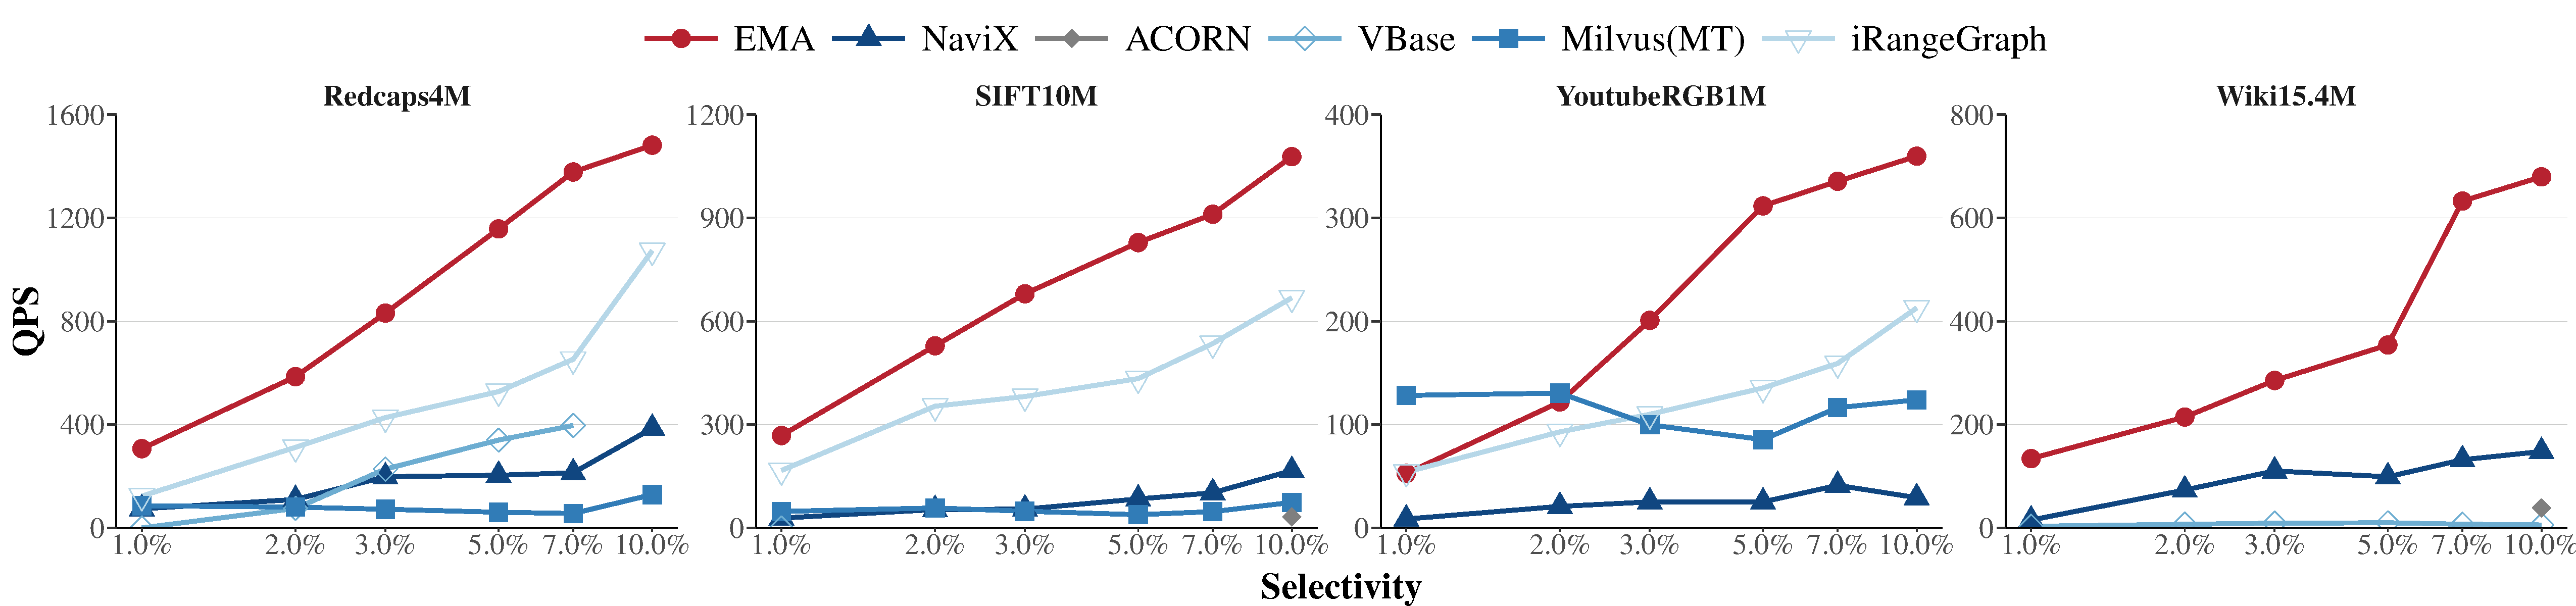
\includegraphics[width=\linewidth]{CH5/figures/range_range_sel_qps.pdf}
    \caption{QPS for range+range biased multi-predicate query at 1\%-10\% selectivity with 95\% recall@10.}
    \label{fig:rangerange}
\end{figure*}

In practice, multi-predicate queries do not always exhibit evenly distributed selectivities across predicates.
We therefore evaluate performance under biased selectivity distributions for range+range queries.
Figure~\ref{fig:rangerange} reports the results at 95\% recall, where the selectivity of the first predicate varies from 55\% to 80\%, while the selectivity of the second
predicate ranges from 1.82\% to 12.5\%.

Compared to evenly distributed queries, \texttt{EMA} exhibits a slight performance degradation under biased selectivity distributions, but still
achieves the best performance in most cases.
This demonstrates that \texttt{EMA} remains robust even when selectivity is highly skewed across predicates.
Predicate-agnostic methods such as \texttt{ACORN} and \texttt{NaviX} are not affected by biased selectivity distributions; however, they still achieve relatively low QPS in
these settings.

We additionally include \texttt{iRangeGraph} in this evaluation as a strong baseline for multi-predicate range queries. \texttt{iRangeGraph} benefits from a high-quality sub-index on the first attribute; however, when the first predicate becomes relatively loose, its search behavior increasingly resembles post-filtering, which limits its effectiveness compared to \texttt{EMA}. 
\texttt{iRangeGraph} failed to construct its index within the 20-hour time limit on Wiki and is not included there.


On the YouTube-RGB dataset, \texttt{Milvus} outperforms \texttt{EMA}, primarily because the dataset size is relatively small and \texttt{Milvus} can effectively leverage parallel linear scan under highly restrictive predicates.
This advantage reflects \texttt{Milvus}'s internal multi-threaded execution.

% \section{Complex Predicate Combination}

% We evaluate EMA on complex Boolean predicates that combine numerical ranges and categorical constraints. Specifically, we use the following predicate:
% \[
% p = \bigl( \texttt{num} \in [a_1, b_1] \;\wedge\; \texttt{cate} \supseteq L_1 \bigr)
% \;\lor\;
% \bigl( \texttt{num} \in [a_1, b_2] \;\wedge\; \texttt{cate} \supseteq L_2 \bigr),
% \]
% which captures a representative class of composed predicates with mixed attribute types and \texttt{AND}/\texttt{OR} operators. We vary the selectivity from 1\% to 10\% while fixing recall at 95\% (recall@10).

% \begin{figure*}[t]
%     \centering
%     \includegraphics[width=\linewidth]{APP/figures/range_label_composite_sel_qps.pdf}
%     \caption{QPS for composed multi-predicate queries at 1\%--10\% selectivity with 95\% recall@10.}
%     \label{fig:comosed}
% \end{figure*}

% Figure~\ref{fig:comosed} reports the results. Under controlled selectivity, EMA maintains stable QPS across different predicate compositions, demonstrating its robustness in handling arbitrary Boolean combinations over numerical and categorical attributes.

\section{Fair Comparison with HNSWLib and NaviX}

Since HNSWLib natively supports filtering, we include it as a baseline to demonstrate the effectiveness of EMA. In addition, NaviX is implemented on top of Faiss, which is generally less competitive than HNSWLib. To ensure a fair comparison, we evaluate (i) naive filtering in HNSWLib and (ii) NaviX implemented on top of HNSWLib.



% Figure~\ref{fig:ablation}

\begin{figure}[t]
  \centering
  \begin{subfigure}[t]{0.6\columnwidth}
    \centering
    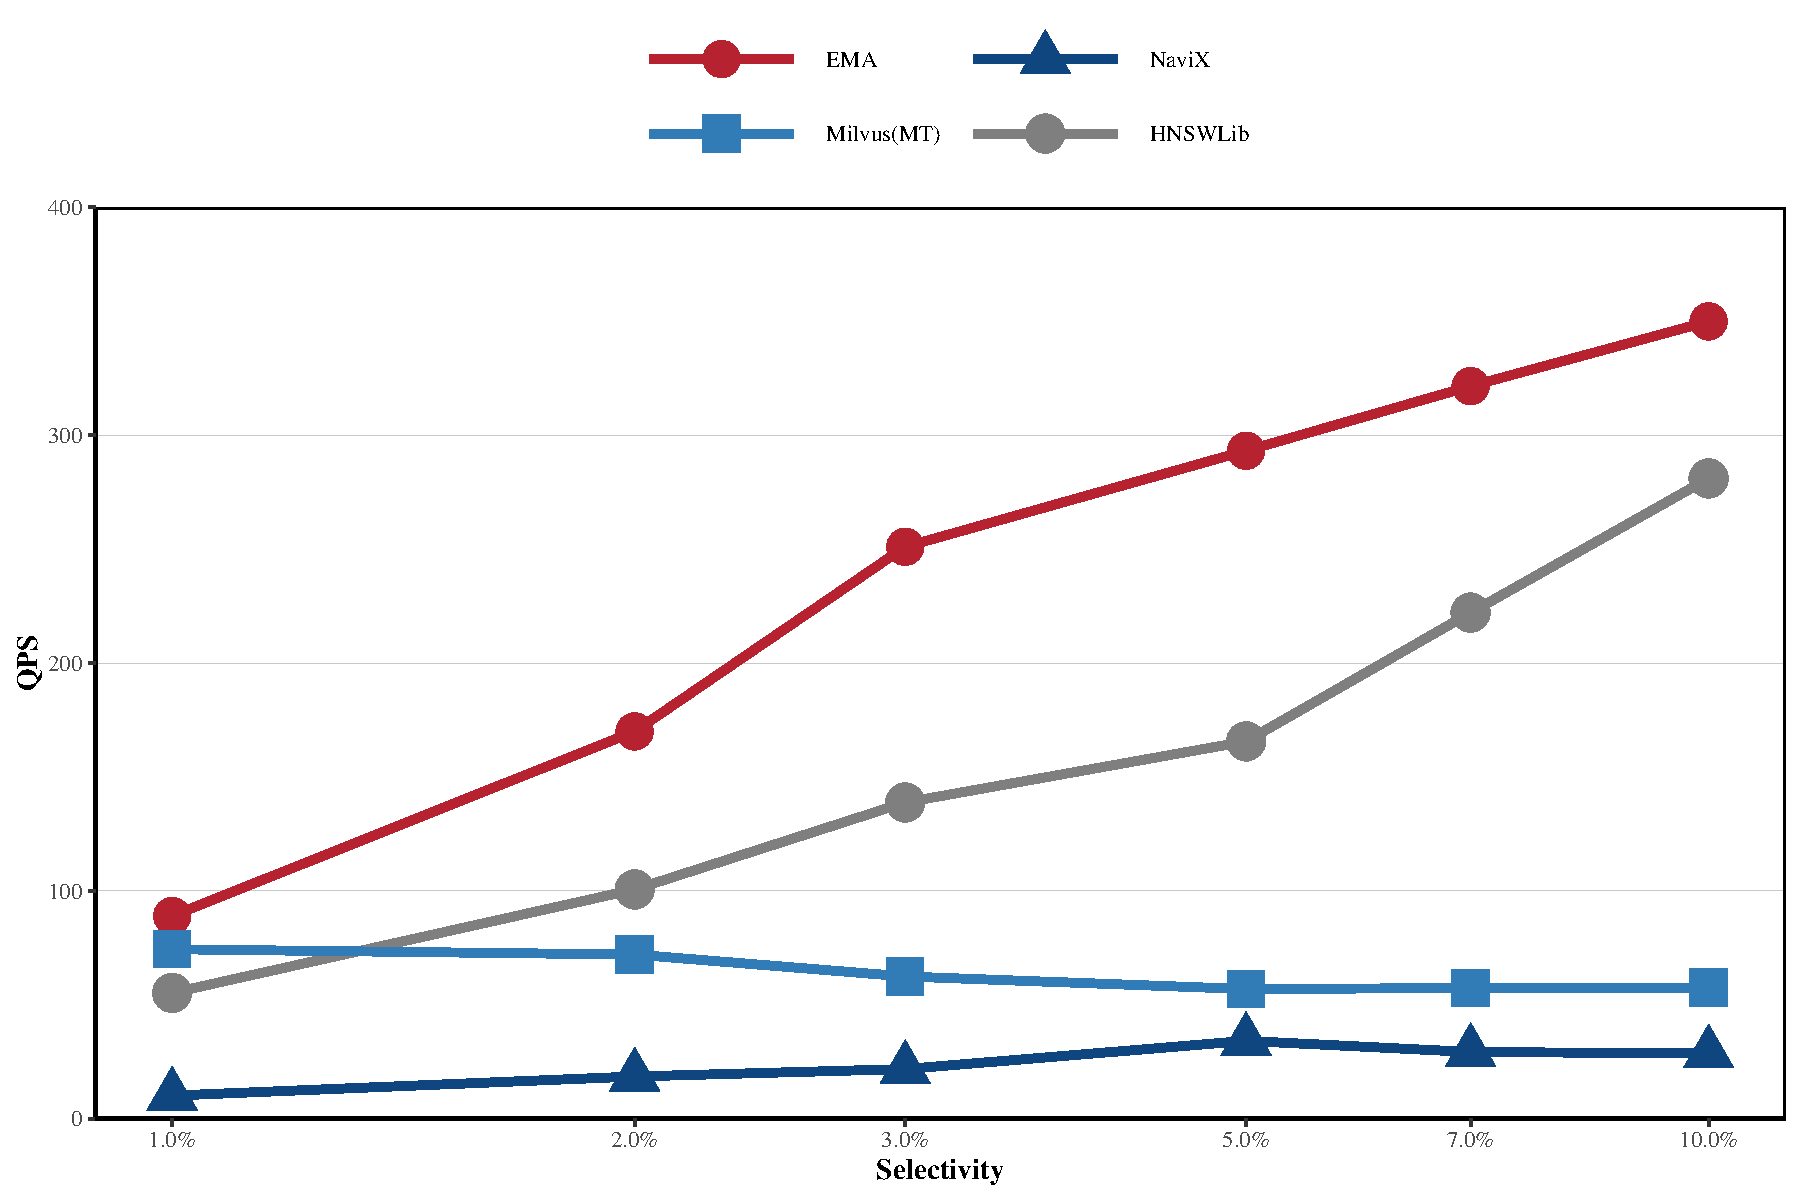
\includegraphics[width=\linewidth]{APP/figures/youtube_sel_qps_with_hnsw.pdf}
    \caption{QPS vs. selectivity on \textbf{YoutubeRGB1M} at 95\% recall.}
    \label{fig:youtube_sel_qps}
  \end{subfigure}\hfil
  \begin{subfigure}[t]{0.6\columnwidth}
    \centering
    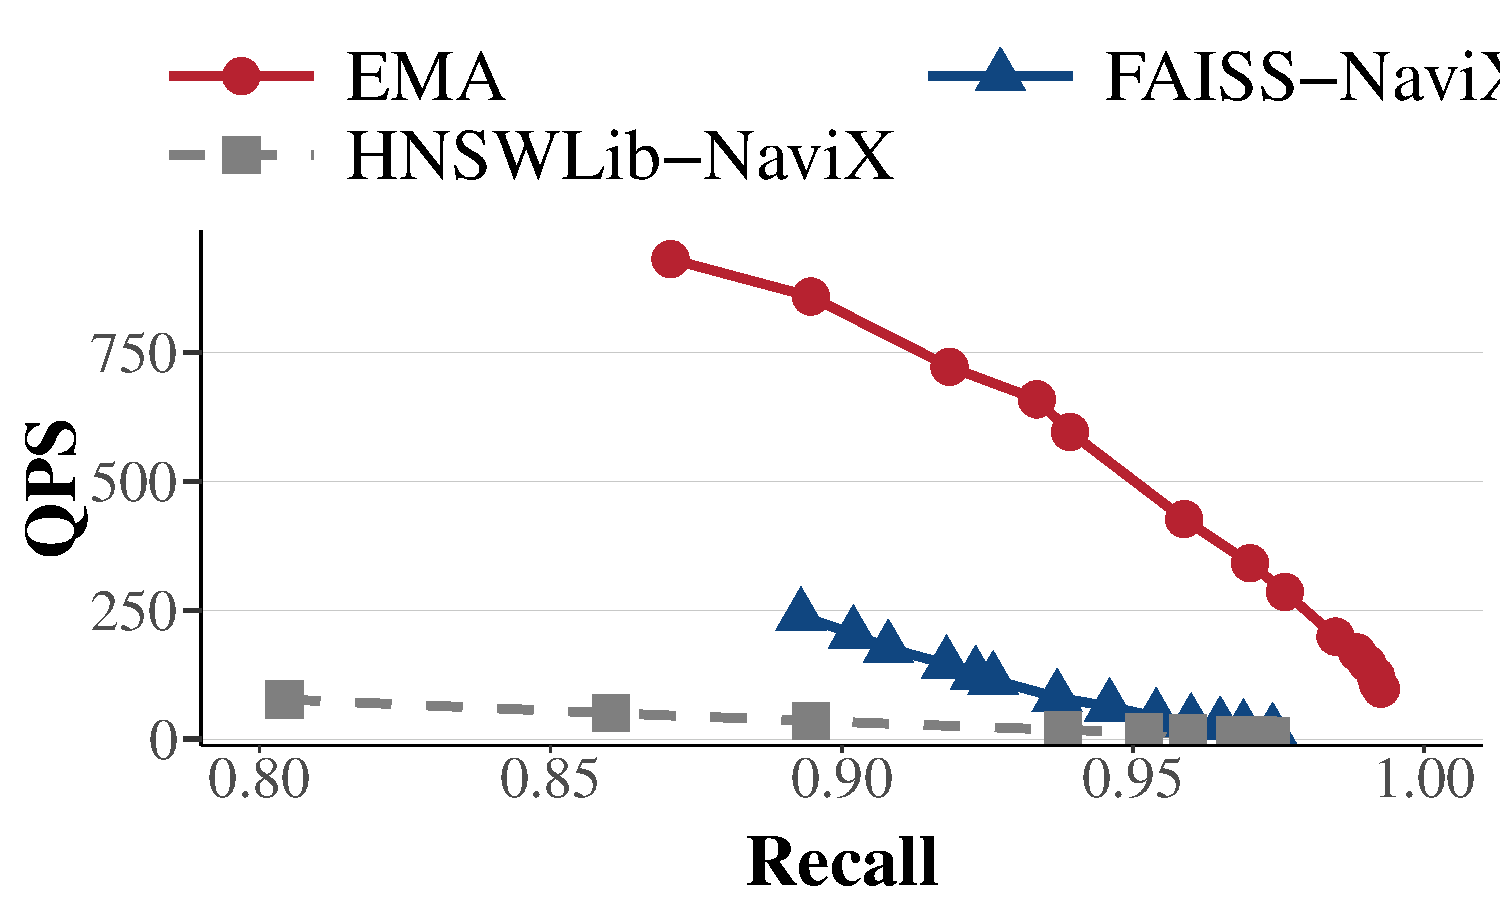
\includegraphics[width=\linewidth]{APP/figures/youtube_recall_qps.pdf}
    \caption{QPS vs. recall on \textbf{YoutubeRGB1M} at 10\% selectivity.}
    \label{fig:youtube_recall_qps}
  \end{subfigure}

  \caption{Experiments across different baselines.}
\end{figure}

Figure~\ref{fig:youtube_sel_qps} shows that EMA consistently outperforms HNSWLib. Moreover, NaviX does not achieve better performance than the HNSWLib baseline.

Figure~\ref{fig:youtube_recall_qps} reports recall--QPS trade-offs at 10\% selectivity. We implement a prototype of NaviX on HNSWLib. Although HNSWLib alone achieves competitive performance, NaviX is sensitive to the underlying index behavior. Compared to Faiss, HNSWLib explores more candidates at the bottom layer; the additional two-hop expansion further amplifies random memory accesses, leading to degraded performance. A detailed analysis will be included in the revision.


\section{Parameter Sensitivity Analysis}

\subsection{Effect of Graph Degree $M$}

\begin{table}[t]
  \caption{HashANN QPS at recall=0.95 on Redcaps\_4M across selectivity and graph degree $M$.}
  \label{tab:m-ablation-redcaps}
  \begin{tabular}{c|cccccc}
    \hline
    \textbf{$M$} & \textbf{1\%} & \textbf{3\%} & \textbf{10\%} & \textbf{40\%} & \textbf{80\%} & \textbf{100\%} \\
    \hline
    16  & \textbf{375}  & \textbf{635}  & 931           & 2200          & 2958          & 3765 \\
    \hline
    32  & 308           & 591           & \textbf{1112} & \textbf{2606} & 3097          & 4904 \\
    \hline
    40  & 330           & 576           & 1073          & 2575          & \textbf{3436} & \textbf{5438} \\
    \hline
    64  & 286           & 533           & 1056          & 2364          & 3399          & 4870 \\
    \hline
    \textbf{best $M$} & 16 & 16 & 32 & 32 & 40 & 40 \\
    \hline
  \end{tabular}
\end{table}

We evaluate the impact of the maximum graph degree $M \in \{16, 32, 40, 64\}$. All other parameters are fixed ($\texttt{ft\_bits}=128$, $\texttt{ft\_routing\_min\_deg}=8$, $ef_c=300$), using single-threaded execution over 1,000 queries. Table~\ref{tab:m-ablation-redcaps} reports QPS at 95\% recall, where bold entries indicate the best $M$ for each selectivity.

Overall, the optimal choice of $M$ depends on selectivity. At low selectivity (1\%--3\%), smaller $M$ performs best, as it reduces neighbor comparison cost and enables faster transition to edge recovery. Increasing $M$ brings no benefit in this regime due to limited candidate expansion. At moderate selectivity (10\%--40\%), $M=32$ achieves the highest QPS, balancing search quality and traversal overhead. At high selectivity (80\%--100\%), $M=40$ becomes optimal, as slightly larger neighborhoods improve connectivity without incurring excessive scanning.

Notably, overly large $M$ (e.g., $64$) consistently underperforms due to increased traversal and unnecessary neighbor evaluation. These results suggest that moderate values of $M$ provide the best trade-off between exploration cost and graph connectivity across selectivity levels.

\subsection{Effect of FT Width (\texttt{ft\_bits})}

\begin{figure}[t]
    \centering
    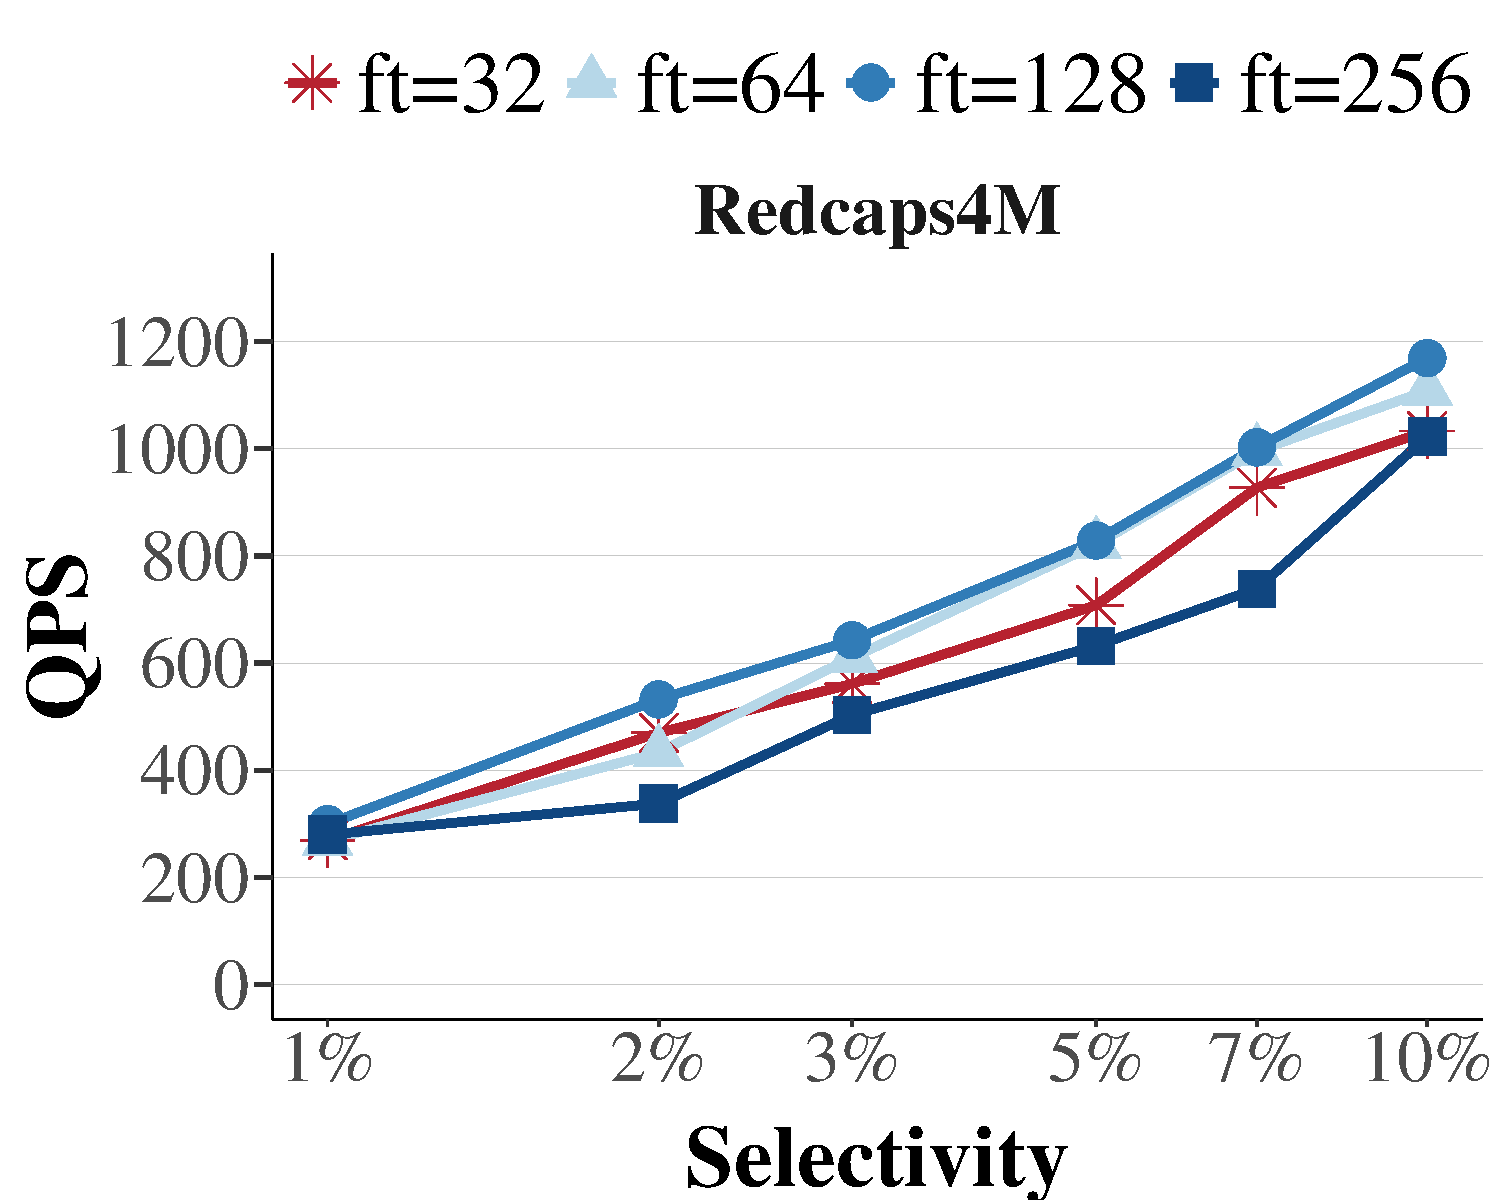
\includegraphics[width=0.8\linewidth]{APP/figures/ablation_ft_bits_redcaps.pdf}
    \caption{Impact of \texttt{ft\_bits} on QPS at 95\% recall across different selectivity levels.}
    \label{fig:ftbits}
\end{figure}

We evaluate the impact of \texttt{ft\_bits} on performance. Figure~\ref{fig:ftbits} reports QPS at 95\% recall across selectivity.

\texttt{ft\_bits}=128 consistently achieves the best performance, improving over 32 bits by 2\%--25\%. Increasing from 32 to 128 bits reduces false positives and improves routing accuracy, while further increasing to 256 bits yields no benefit due to the enlarged memory footprint, which increases cache access cost and dominates query latency. \texttt{ft\_bits}=64 provides a reasonable trade-off but remains slightly inferior to 128 bits. Thus, we use \texttt{ft\_bits}=128 by default.


\subsection{Effect of Edge Recovery Threshold (\texttt{min\_deg})}

\begin{figure}[t]
    \centering
    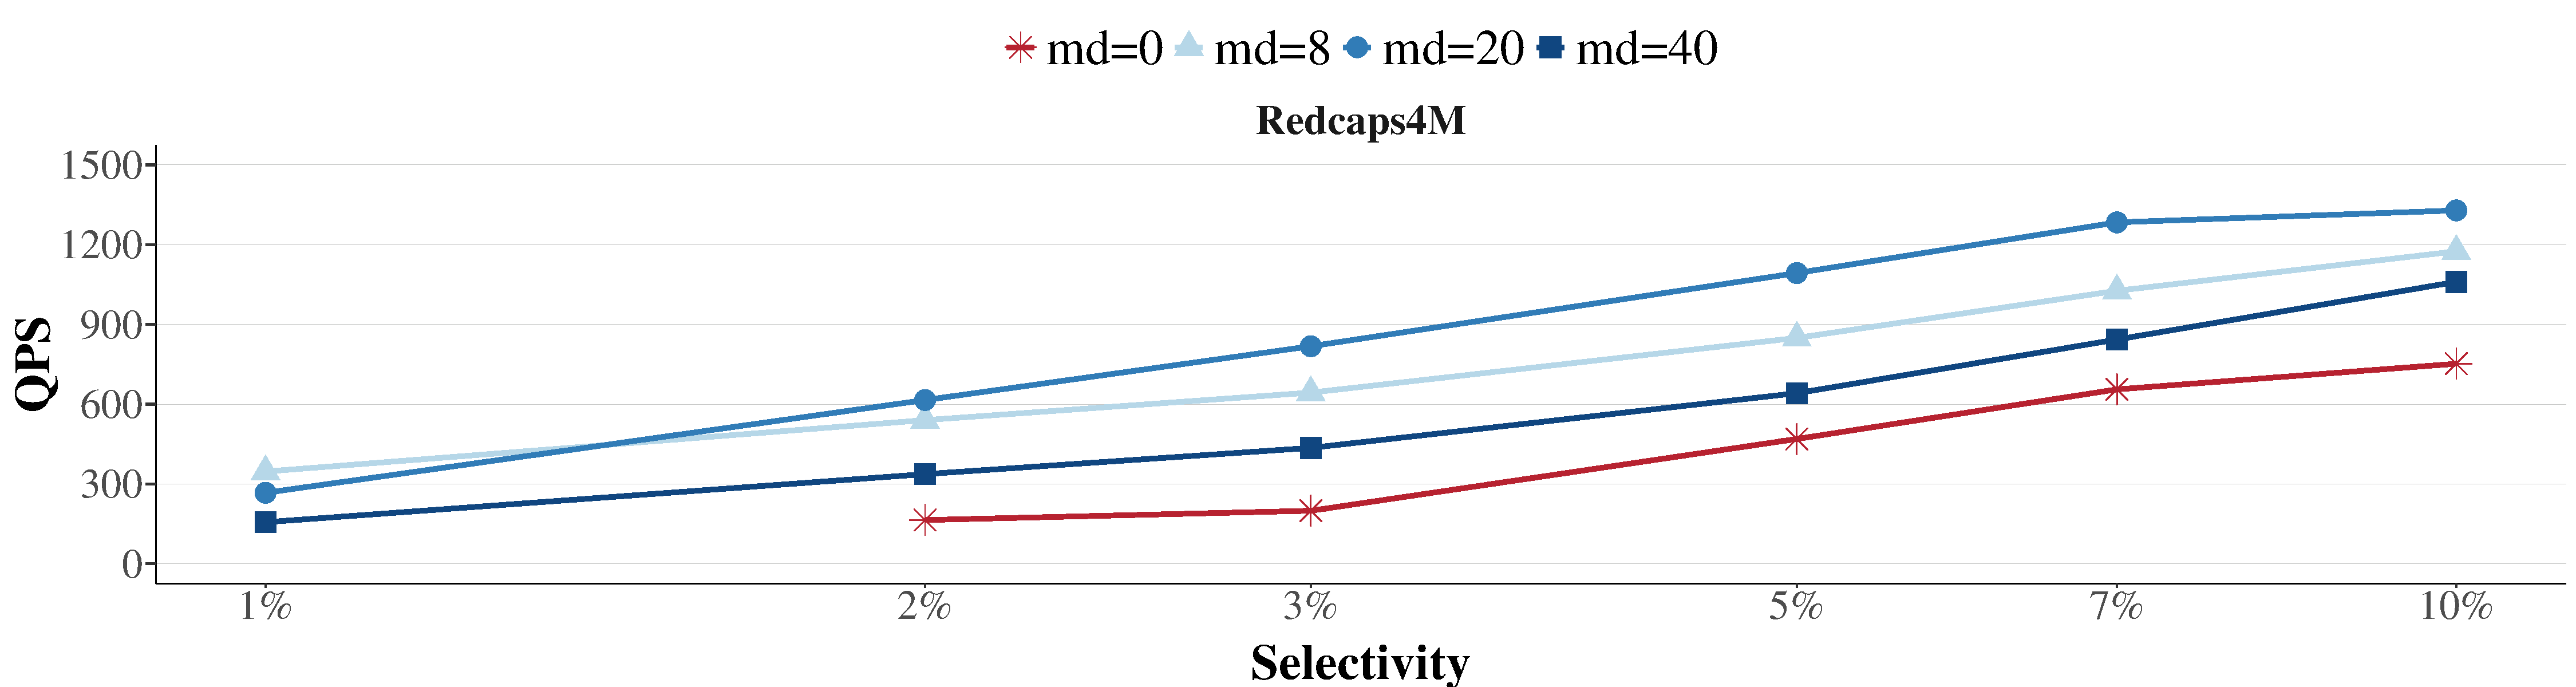
\includegraphics[width=0.8\linewidth]{APP/figures/ablation_min_deg_redcaps.pdf}
    \caption{Impact of \texttt{min\_deg} on QPS at 95\% recall across different min\_deg levels.}
    \label{fig:md_ablation}
\end{figure}

We evaluate the effect of the minimum degree in edge recovery (\texttt{min\_deg}). Figure~\ref{fig:md_ablation} reports QPS at 95\% recall under varying selectivity.

Performance exhibits a clear peak at moderate \texttt{min\_deg}. Under $M{=}40$ (level-0 degree $\approx 80$), the optimal range lies between 15 and 20, achieving the highest QPS across selectivities. Increasing \texttt{min\_deg} beyond this range leads to a sharp degradation (30\%--55\%), as the search progressively approaches post-filtering behavior.

When \texttt{min\_deg} becomes large (e.g., $\geq 40$), the effective neighborhood is saturated, and traversal degenerates to visiting nearly all neighbors, effectively discarding FT-based routing. This regime is consistently slower (up to 2.9$\times$) than the optimal setting, highlighting that FT routing is effective only when \texttt{min\_deg} is properly constrained.

Overall, these results reveal a narrow operating region (\texttt{min\_deg} $\in [8, 20]$) where EMA significantly outperforms post-filtering, confirming that controlled edge recovery is critical to preserving routing efficiency.


\begin{table}[t]
    \caption{FPR on Redcaps1M.}
    \label{tab:fpr}
    \centering
    \begin{tabular}{c|c|c}
        \hline
        \multirow{2}{*}{\textbf{Selectivity}}
          & \multicolumn{2}{c}{\textbf{FPR}} \\
        \cline{2-3}
        & \textbf{Range+Label} &\textbf{Range} \\
        \hline
        \hline
          1\% & 3.84\% & 2.99\% \\
        \hline
          5\% & 4.80\% & 3.67\%  \\
        \hline
          10\% & 5.41\%  & 4.27\% \\
        \hline
          20\% & 6.20\% & 5.18\%  \\
        \hline
          60\% & 7.97\% & 7.71\%  \\
        \hline
    \end{tabular}
    % \setlength{\textfloatsep}{6pt}
\end{table}


\section{Other Studies}
\subsection{False positive rate of the Marker.}
The effectiveness of \texttt{EMA} depends on the accuracy of the Marker, as a lower false positive rate (FPR) reduces unnecessary candidate exploration during joint filtering.
Table~\ref{tab:fpr} reports the FPR on RedCaps1M across selectivity levels ranging from 1\% to 60\%.

% The reported false positive rates are measured with edge recovery disabled and a fixed $efs$, to isolate the accuracy of the Marker itself. Across this range of selectivities, the FPR remains below 10\% for both range+label and range-only queries, and increases moderately with selectivity.

The reported false positive rates are measured with edge recovery disabled and a fixed search parameter ($efs$), so as to isolate the accuracy of the Marker itself.
Across this broad range of selectivities, the FPR consistently remains below 10\% for both range+label and range-only queries. As selectivity increases, the FPR grows moderately, which is expected as filtering becomes less restrictive.

Overall, these results indicate that the Marker provides effective pre-checking with a low and stable false positive rate, supporting efficient query processing across different selectivity regimes.


% \begin{minipage}{0.48\textwidth}
\begin{figure}[t]
    \centering
    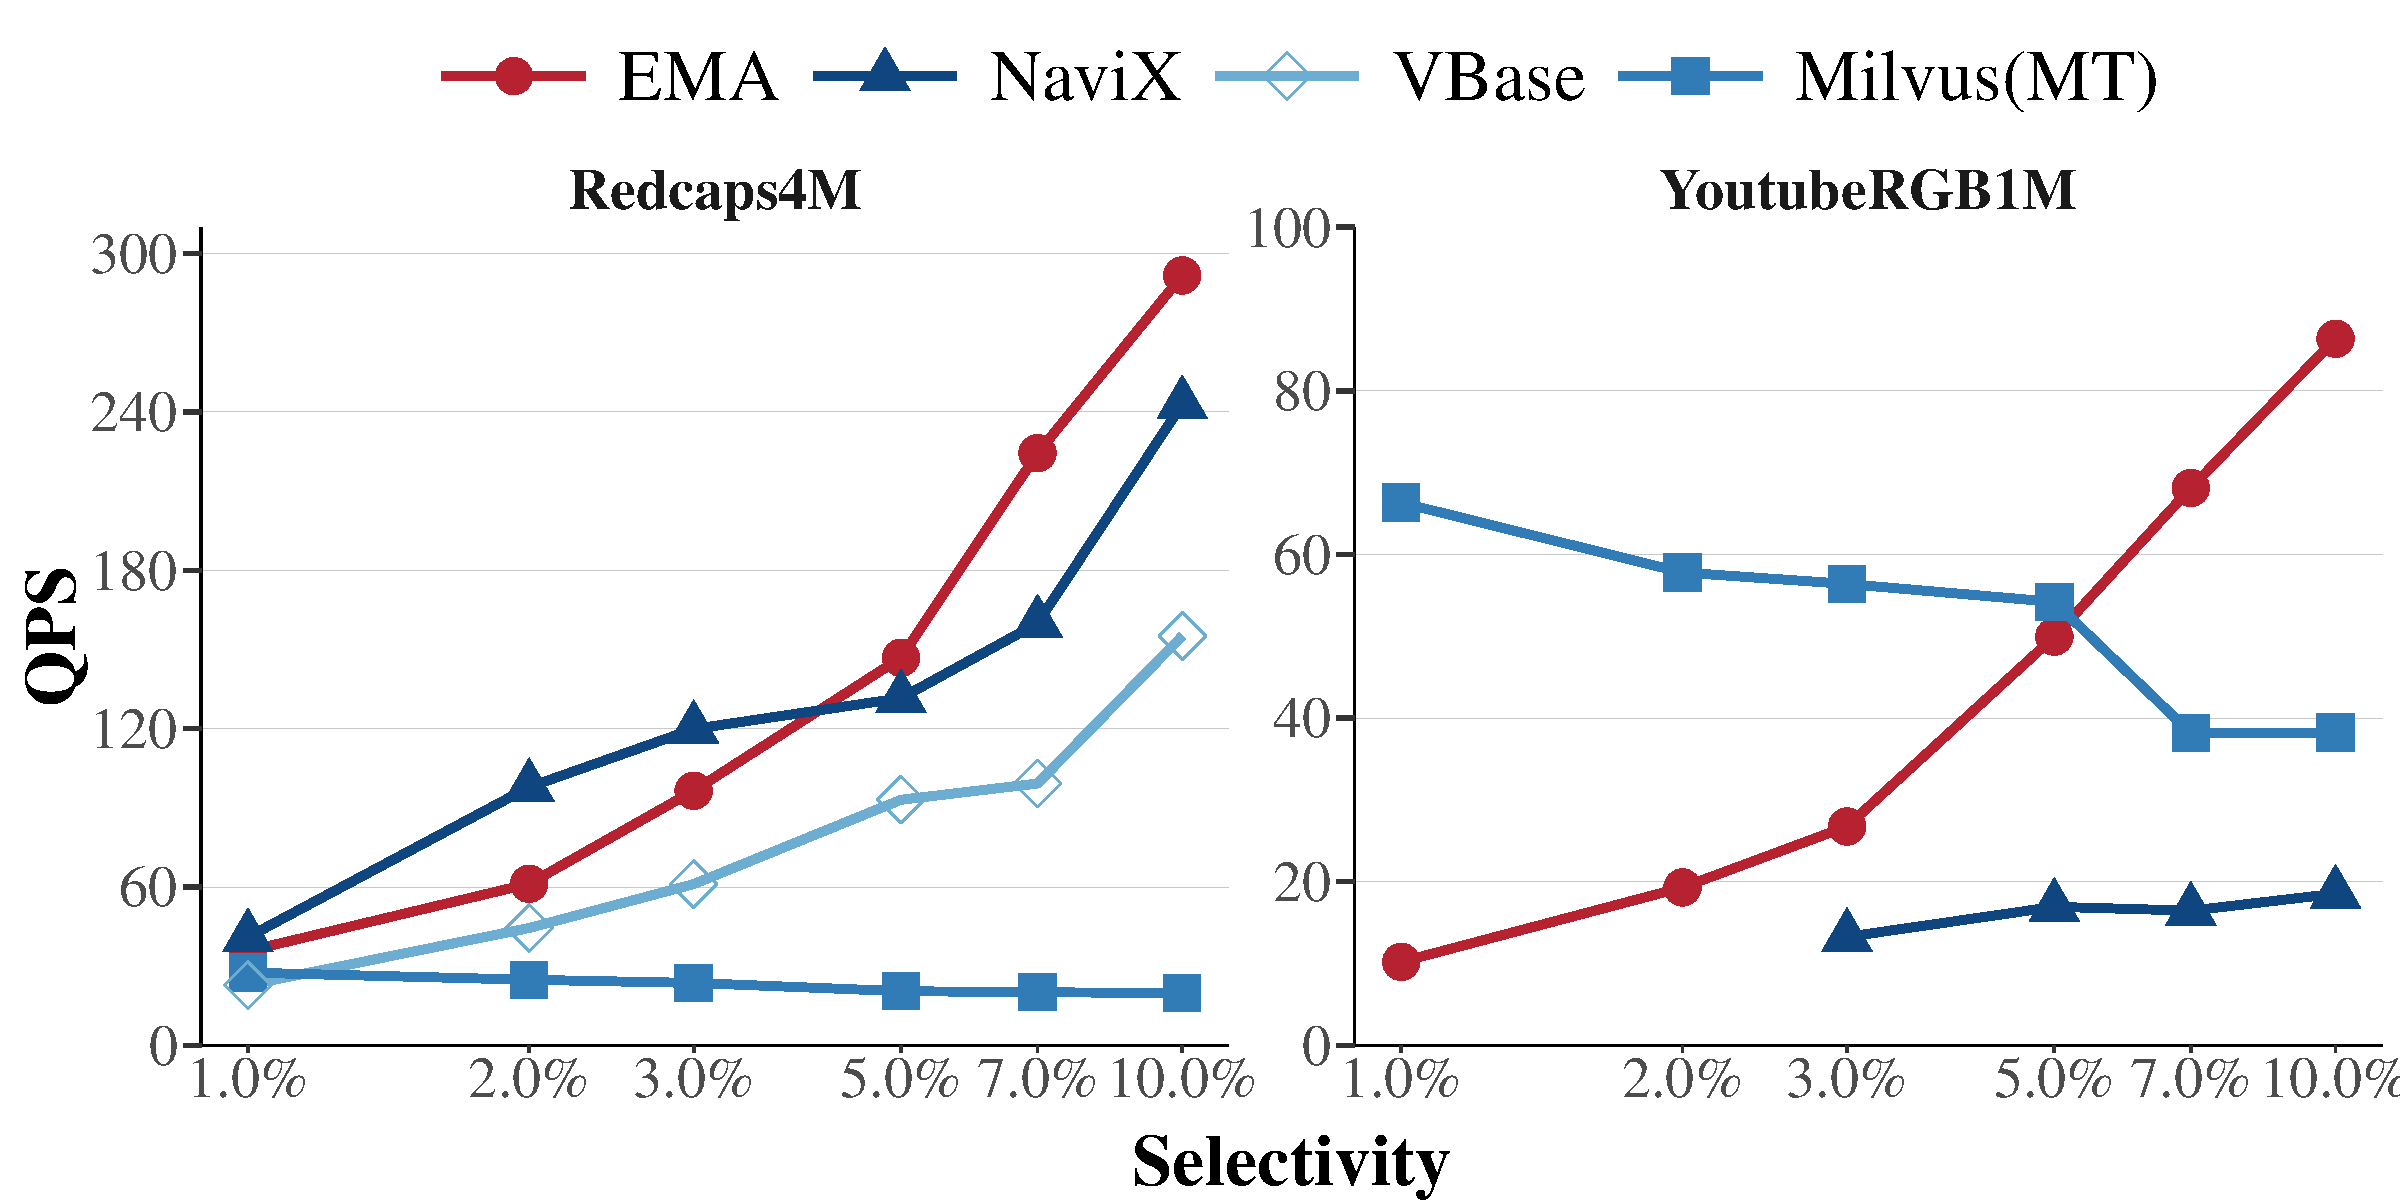
\includegraphics[width=\linewidth]{CH5/figures/range_label_sel_qps_k100.pdf}
    \caption{Label-range query at 95\% recall@100.}
    \label{fig:k100}
\end{figure}
% \end{minipage}


\subsection{Performance at 95\% Recall@100.}
Figure~\ref{fig:k100} reports the QPS under the $R@100$ setting. While \texttt{EMA} exhibits slightly lower throughput in some cases, it is important to note that \texttt{EMA} consistently achieves a higher recall level (approximately 99\%) compared to the 95\% recall target used by other methods.

This difference arises from the more conservative convergence criteria adopted by \texttt{EMA}, which prioritize retrieval accuracy and result stability.
As a result, the reported throughput reflects a stricter recall requirement, highlighting a trade-off between efficiency and accuracy under the $Rrecall@100$
evaluation.

\subsection{Ablation study.}

\begin{figure}[t]
\centering
\begin{minipage}{0.48\textwidth}
% \begin{figure}[t]
    \centering
    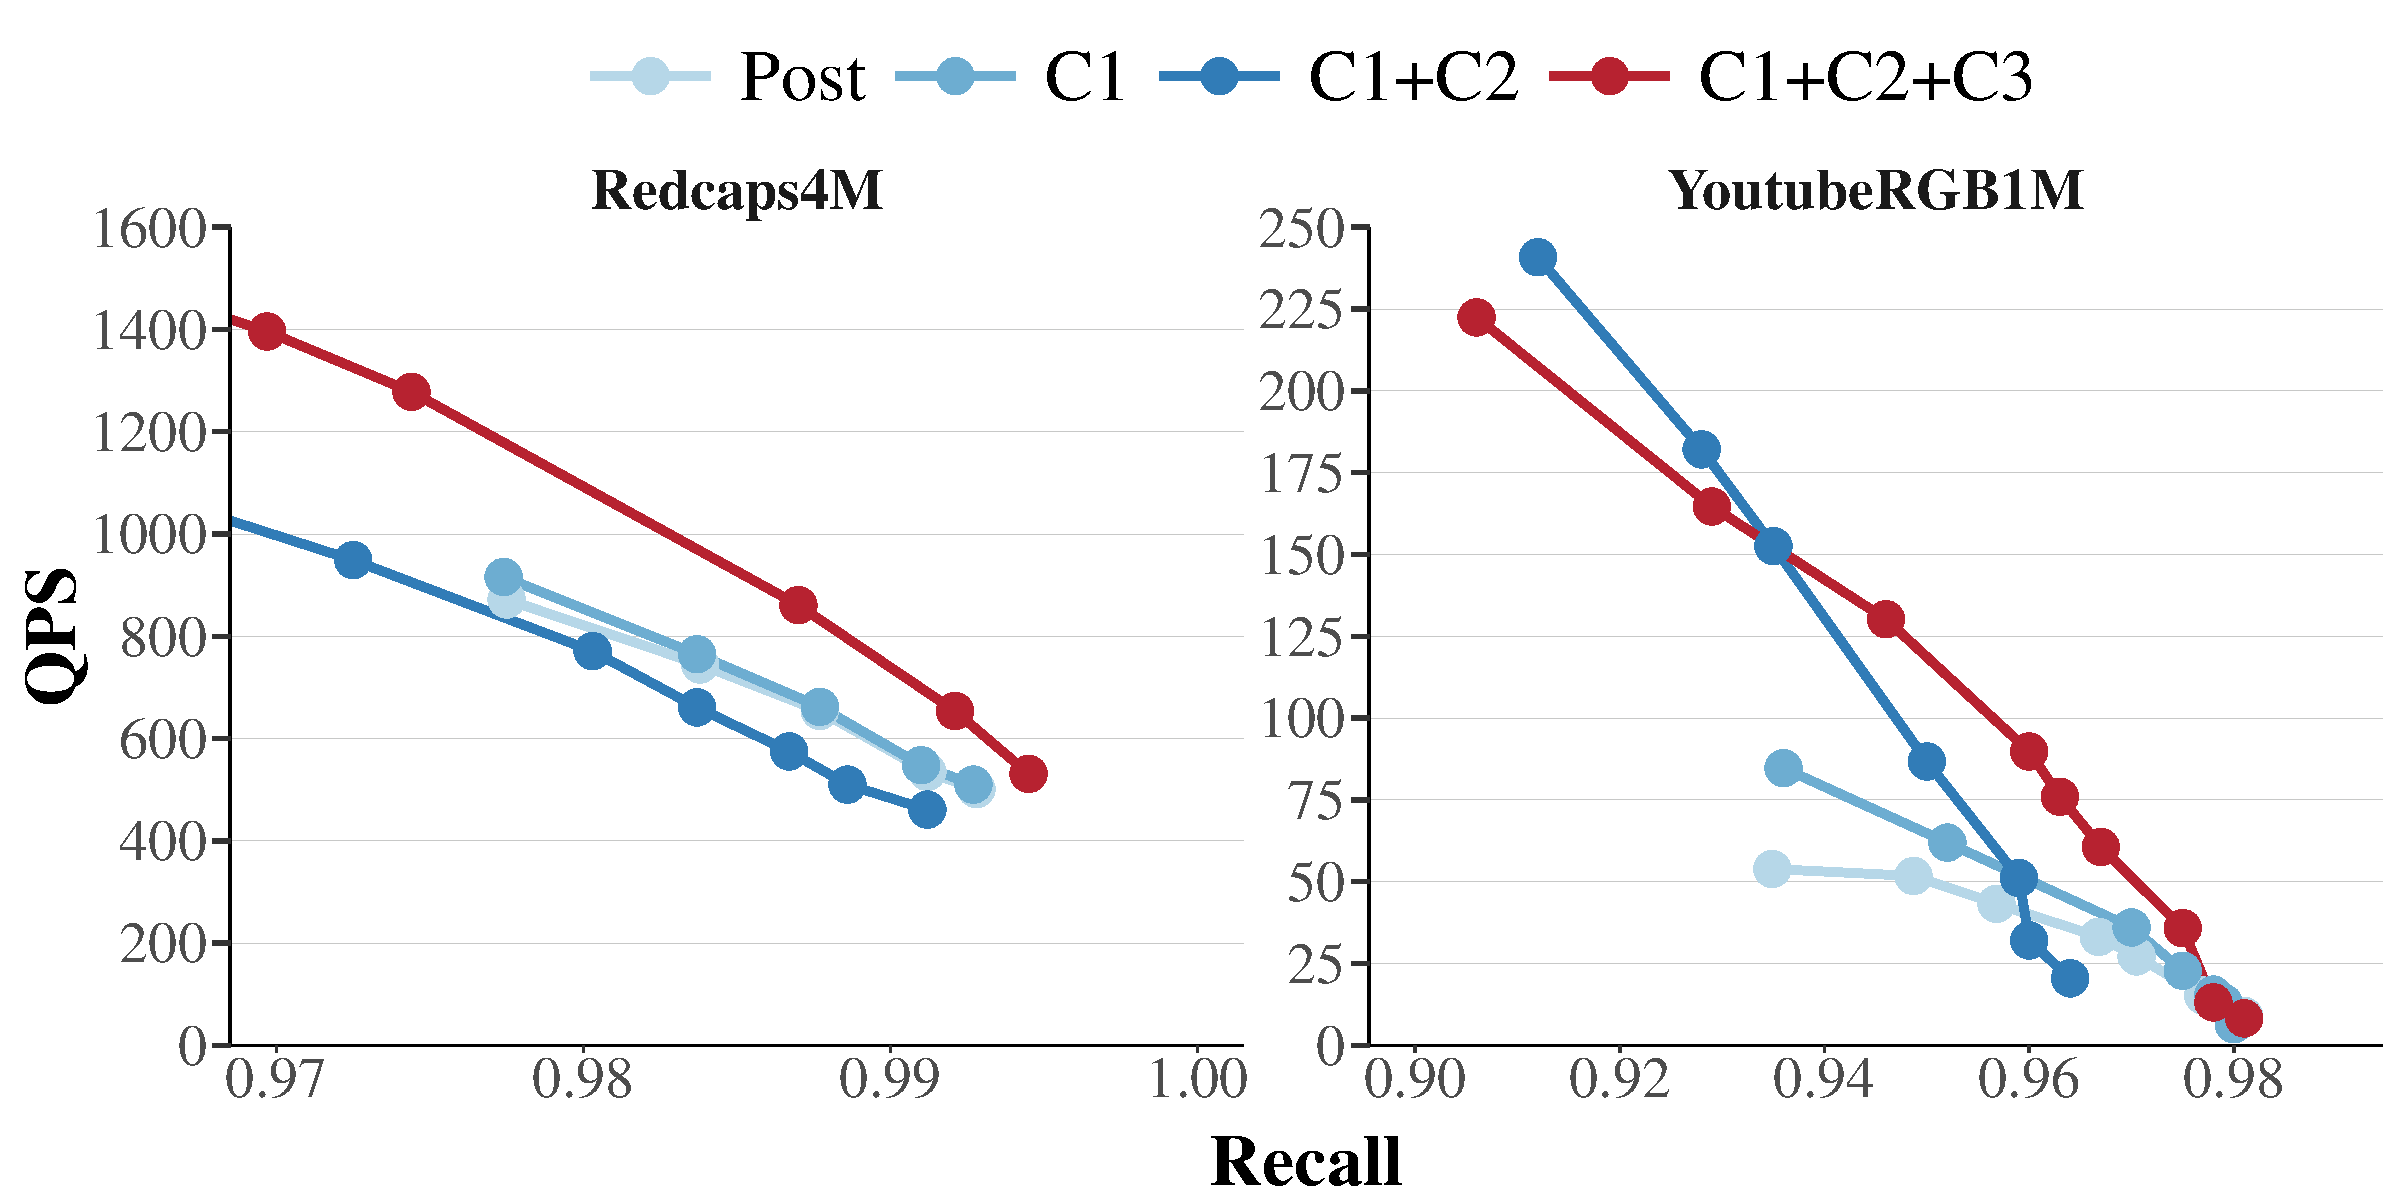
\includegraphics[width=\linewidth]{CH5/figures/abla.pdf}
    \caption{Ablation study on Redcaps and Youtube-RGB.}
    
    \label{fig:ablation}
% \end{figure}
\end{minipage}
\hfill
% \begin{minipage}{0.48\textwidth}
% % \begin{figure}[t]
%     \centering
%     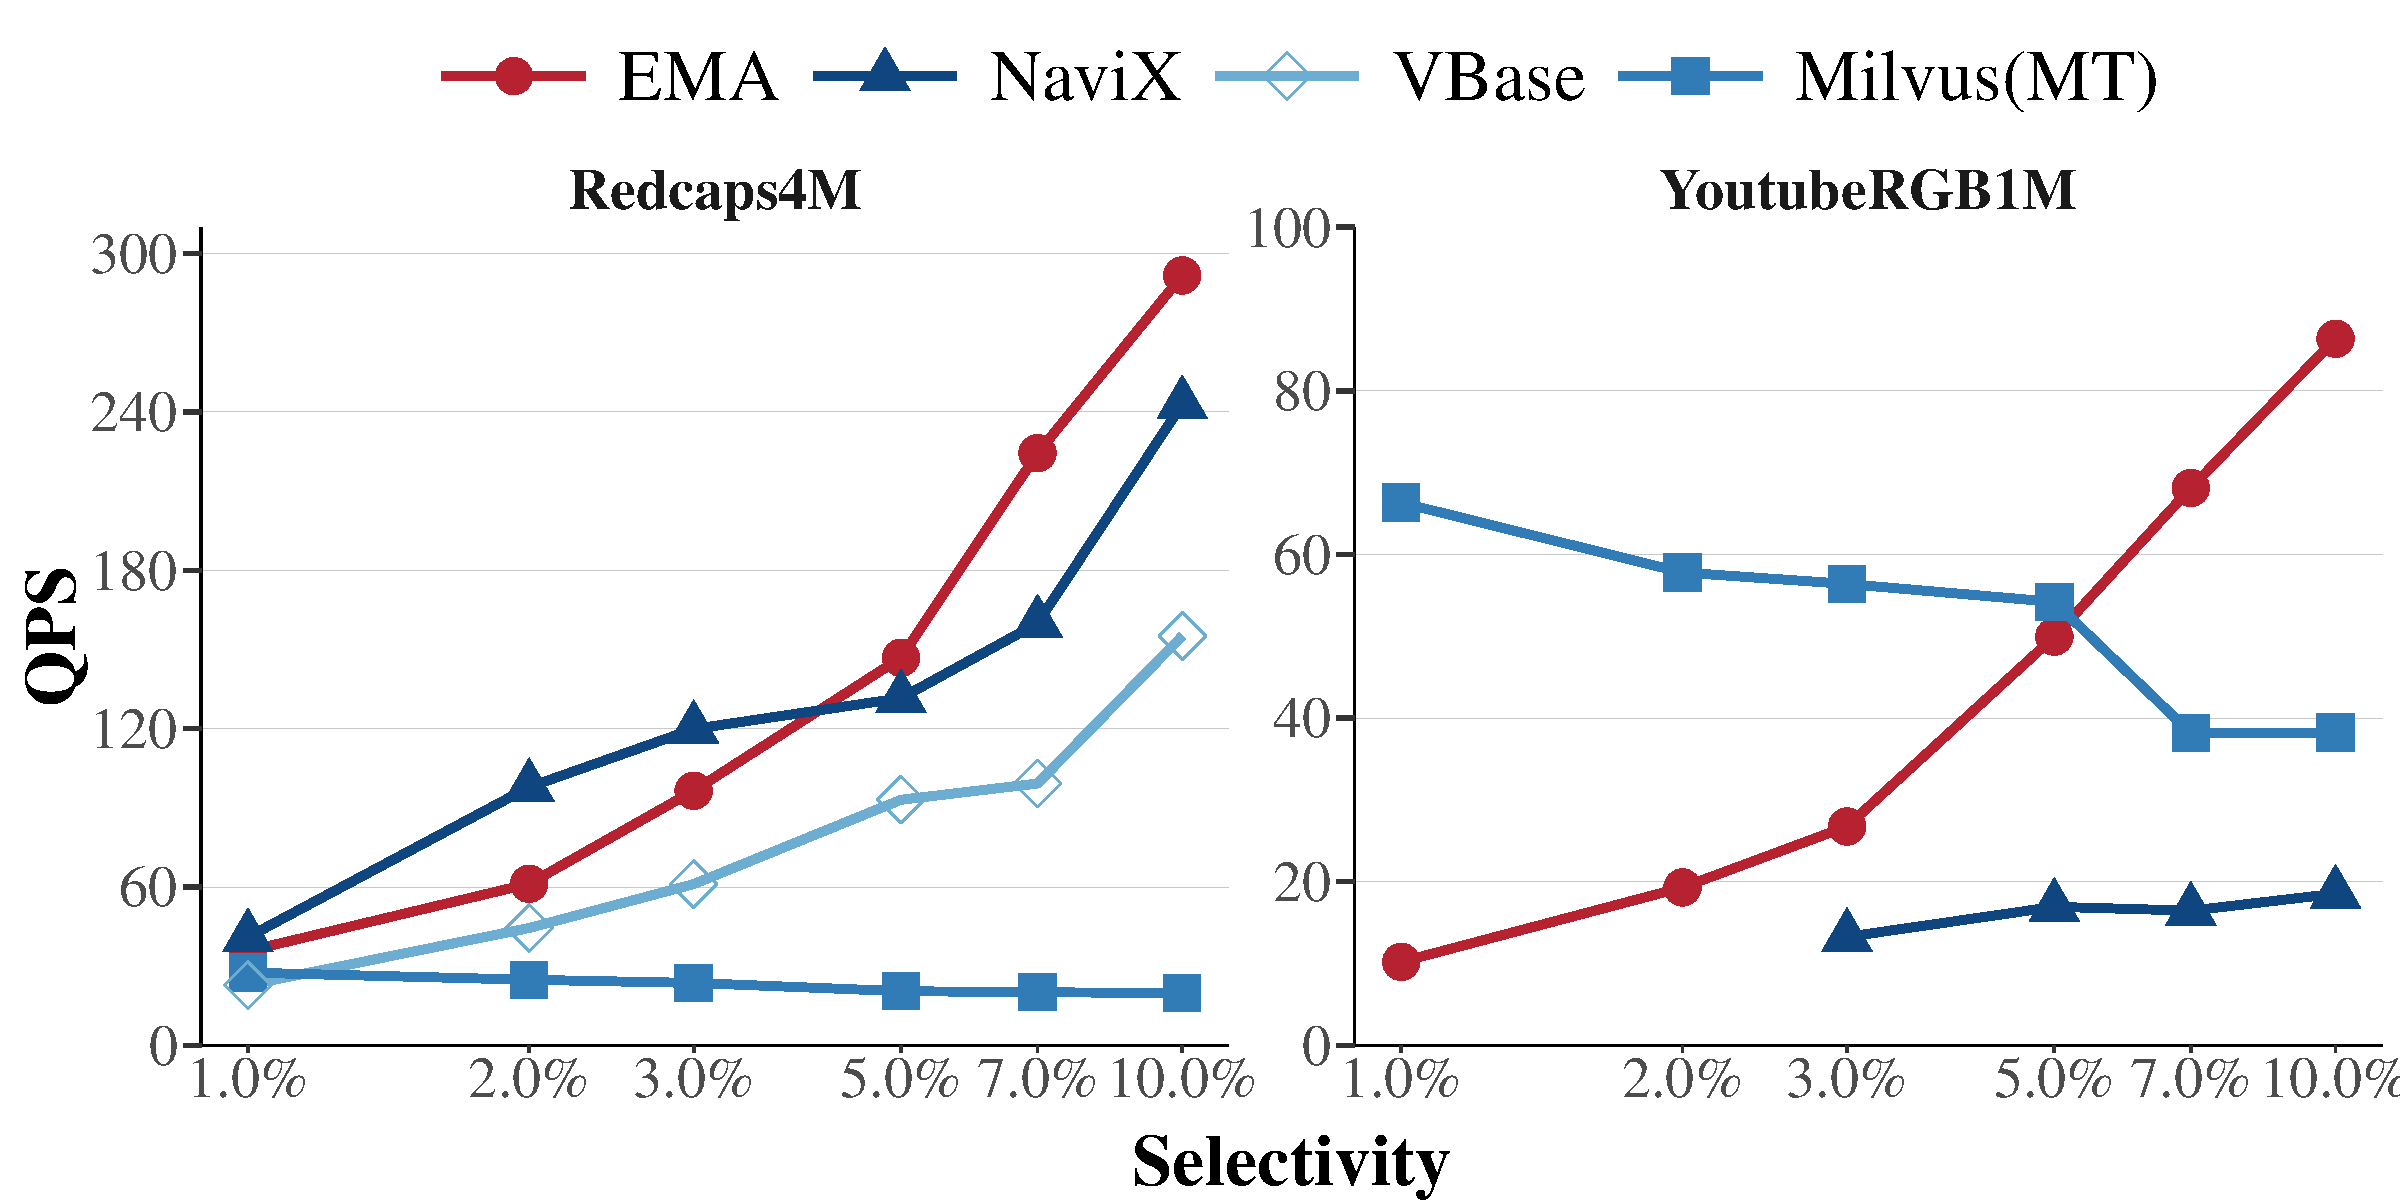
\includegraphics[width=\linewidth]{CH5/figures/range_label_sel_qps_k100.pdf}
%     \caption{Label-range query at 95\% recall@100.}
%     \label{fig:k100}
% % \end{figure}
% \end{minipage}

\end{figure}
% \vspace{-5mm}
% \textbf{Ablation study.}
Building upon the classic post-filtering approach on HNSW, we decompose our method
into three key components:
(1) diversity-aware pruning (C1),
(2) joint filtering with Markers (C2), and
(3) neighbor recovery under low selectivity (C3).

Figure~\ref{fig:ablation} presents an ablation study on the YouTube-RGB dataset under 1\% selectivity and the RedCaps dataset under 10\% selectivity with both range and label constraints. 
Compared with the original HNSW post-filtering baseline, each proposed component consistently improves retrieval performance, and their combination yields the best overall results. 
In particular, introducing the Marker slightly reduces QPS at high recall targets, but yields a noticeable performance improvement at lower recall levels (around 92\%). This improvement indicates that the Marker effectively prunes unnecessary traversals while preserving sufficient candidates, providing a strong foundation for further performance gains when combined with the edge recovery strategy.
